
\definecolor{mygreen}{rgb}{0,0.6,0}

\pgfdeclarelayer{background}
\pgfsetlayers{background,main}

\tikzstyle{vertex}=[circle,fill=black!25,minimum size=20pt,inner sep=0pt]
\tikzstyle{selected vertex} = [vertex, fill=red!24]
\tikzstyle{select vertex} = [vertex, fill=blue!24]
\tikzstyle{selectx vertex} = [vertex, fill=green!24]
\tikzstyle{edge} = [draw,thick,-]
\tikzstyle{selected edge} = [draw,line width=5pt,-,red!50]


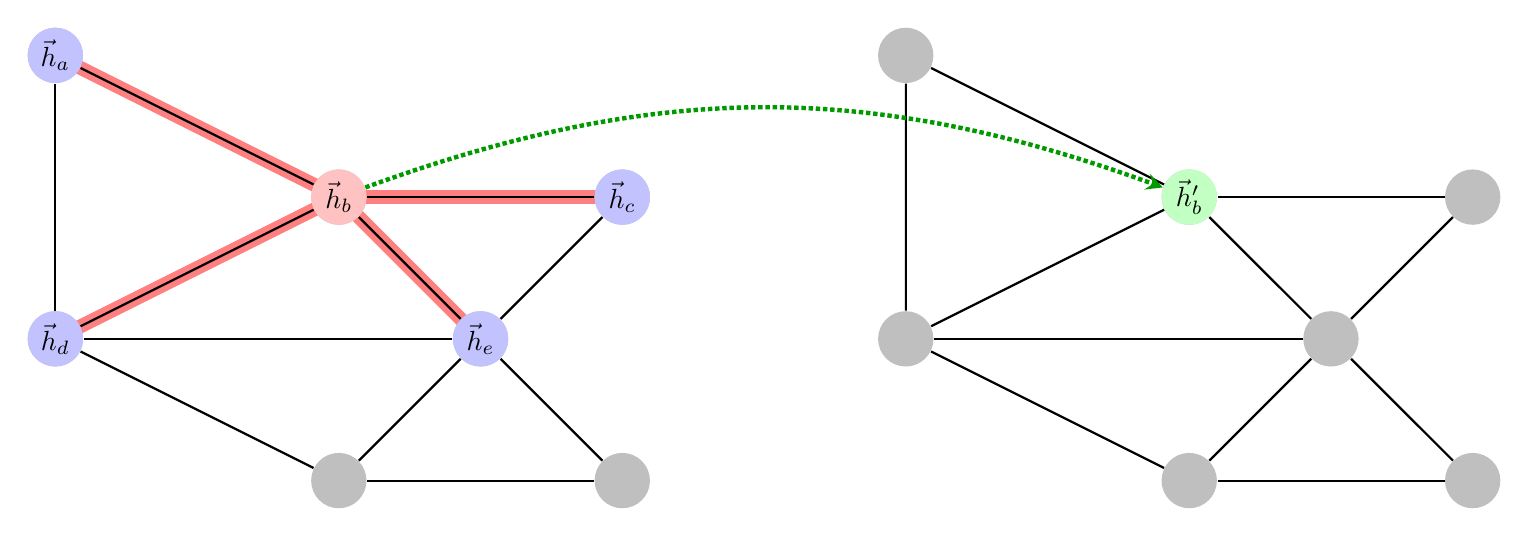
\begin{tikzpicture}[scale=1.8, auto,swap]
    \foreach \pos/\name in {{(0,2)/a}, {(2,1)/b}, {(4,1)/c},
                            {(0,0)/d}, {(3,0)/e}, {(2,-1)/f}, {(4,-1)/g}}
        \node[vertex] (\name) at \pos {};
        
    \foreach \source/ \dest /\weight in {b/a/7, c/b/8,d/a/5,d/b/9,
                                         e/b/7, e/c/5,e/d/15,
                                         f/d/6,f/e/8,
                                         g/e/9,g/f/11}
        \path[edge] (\source) -- (\dest);
         
    \foreach \vertex / \fr in {b/4}
        \path node[selected vertex] at (\vertex) {$\vec{h}_b$};
    \foreach \vertex / \fr in {a/4, c/4, d/4, e/5}
        \path node[select vertex] at (\vertex) {$\vec{h}_{\vertex}$};
    \begin{pgfonlayer}{background}
        \foreach \source / \dest in {b/c,d/b,a/b,b/e}
            \path[selected edge] (\source.center) -- (\dest.center);
    \end{pgfonlayer}
    
    \foreach \pos/\name in {{(6,2)/a1}, {(8,1)/b1}, {(10,1)/c1},
                            {(6,0)/d1}, {(9,0)/e1}, {(8,-1)/f1}, {(10,-1)/g1}}
        \node[vertex] (\name) at \pos {};
    \foreach \source/ \dest /\weight in {b1/a1/7, c1/b1/8,d1/a1/5,d1/b1/9,
                                         e1/b1/7, e1/c1/5,e1/d1/15,
                                         f1/d1/6,f1/e1/8,
                                         g1/e1/9,g1/f1/11}
        \path[edge] (\source) -- (\dest);
    \foreach \vertex / \fr in {b1/4}
        \path node[selectx vertex] at (\vertex) {$\vec{h}'_b$};
        
    \draw[-stealth, densely dotted, ultra thick, mygreen] (b) edge[bend left=20] (b1);
\end{tikzpicture}

